\documentclass[a4paper,12pt]{extreport}
\usepackage[left=20mm,right=10mm,top=20mm,bottom=20mm]{geometry}
% \parindent 1.25cm
% \linespread{1.5}

\usepackage{cmap}
\usepackage{lipsum}

\usepackage[utf8]{inputenc}
\usepackage[T2A]{fontenc}
\usepackage[english,russian]{babel}
\usepackage{fontspec}
\setmainfont{Times New Roman}
\setmonofont{Consolas}

\usepackage{color}
\usepackage{listings}

\lstset{ %
    language=python,                % выбор языка для подсветки (здесь это С)
    basicstyle=\small\ttfamily,   % размер и начертание шрифта для подсветки кода
    numbers=left,                 % где поставить нумерацию строк (слева\справа)
    numberstyle=\tiny,            % размер шрифта для номеров строк
    stepnumber=1,                 % размер шага между двумя номерами строк
    firstnumber=1,
    numberfirstline=true
    numbersep=5pt,                % как далеко отстоят номера строк от подсвечиваемого кода
    backgroundcolor=\color{white},% цвет фона подсветки - используем \usepackage{color}
    showspaces=false,             % показывать или нет пробелы специальными отступами
    showstringspaces=false,       % показывать или нет пробелы в строках
    showtabs=false,               % показывать или нет табуляцию в строках
    frame=single,                 % рисовать рамку вокруг кода
    tabsize=2,                    % размер табуляции по умолчанию равен 2 пробелам
    captionpos=t,                 % позиция заголовка вверху [t] или внизу [b]
    breaklines=true,              % автоматически переносить строки (да\нет)
    breakatwhitespace=false      % переносить строки только если есть пробел
}

\usepackage{graphicx}
\usepackage{float}
\usepackage{subcaption}
\usepackage{xltabular, tabularx}

\usepackage[raggedright]{titlesec} % заголовки

\newcounter{slide}
\setcounter{slide}{1}

% \newcommand{\customparagraph}{(\arabic{slide}) \theparagraph}

\titleformat{\paragraph}[block]{\bfseries}{\theparagraph}{{|}}{(Слайд \arabic{slide}) }[\addtocounter{slide}{1}]
\titlespacing{\paragraph}{0pt}{10pt}{0pt}

\begin{document}

\paragraph{Титульник}

Добрый день, уважаемые члены комиссии, меня зовут Поздняков Артемий Анатольевич
и я хочу представить выпускную квалификационную работу бакалавра на тему
''Сравнение методов сжатия атрибутов облаков точек''. Научным руководителем
данной работы является Федоров Станислав Алексеевич.

\paragraph{Актуальность}

Растущая популярность технологий компьютерного зрения и расширенной реальности
влечёт за собой потребность в способах компактного хранения и передачи облаков
точек. В настоящее время появляется большое количество кодеков, предназначенных
для сжатия облаков точек и их атрибутов (PCC-кодеков), что делает актуальной
задачей разработку программы для оценки работы PCC-кодеков. Подобная программа
может быть использована исследователями для подсчёта метрик разрабатываемых ими
кодеков.

\paragraph{Цели и задачи}

\textbf{Цель работы} - разработка подхода к сравнению методов сжатия атрибутов
облаков точек. В рамках данной работы необходимо решить следующие задачи:

\begin{itemize}
    \item Проанализировать системы оценки качества сжатия облаков точек
    \item Изучить релевантные метрики, отображающие эффективность и качество
    сжатия атрибутов облаков точек
    \item Разработать программу подсчёта метрик
    \item Получить метрики для отобранных PCC-кодеков
    \item Проанализировать результаты работы
\end{itemize}

\paragraph{Более расширенное введение, классификация метрик}

Сравнение кодеков будет осуществляться следующим образом: возьмем некоторое
контрольное облако точек, осуществим его компрессию и декомпрессию с помощью
некоторого кодека $C$, полученное в результате декомпрессии облако точек назовём
реконструированным облаком точек. Показателем качества сжатия данного облака
точек, то есть качественной оценкой работы кодека, будут являться значения
отобранных метрик для пары оригинальное и реконструированное облако.

% \paragraph{GeoCNN geo\_dist}

% \lipsum[1][1-4]

% \paragraph{mpeg-pcc-dmetric}

% \lipsum[1][1-4]

% \paragraph{PCCArena}

% \lipsum[1][1-4]

\paragraph{Сравнение указанных альтернативных решений}

Среди существующих решений, предназначенных для данной задачи, можно отметить
системы оценки mpeg\_pcc\_dmetric от MPEG и geo\_dist от авторов кодека
GeoCNNv1.

\begin{xltabular}{\linewidth}{|l|X|X|}
    \hline
    & mpeg\_pcc\_dmetric & geo\_dist \\
    \hline
    Полнота метрик & +- & +- \\
    \hline
    Оценка искажения атрибутов & + & - \\
    \hline
    Поддерживаемость & + & - \\
    \hline
    Возможность расширения & - & - \\
    \hline
    Открытый исх. код & - & - \\
    \hline
    \caption{
        Характеристики различных рассмотренных систем.
        \label{tab:systems_comparison}
    } \\
\end{xltabular}

На таблице \ref{tab:systems_comparison} приведены характеристики данных систем
оценки. Здесь, под полнотой метрик подразумевается возможность подсчёта
среднеквадратичной ошибки, отношения пикового сигнала к шуму, а также значения
данных метрик, проецированные вдоль нормалей точек (нормаль точки - нормаль к
плоскости, на которой лежит точка). Что касается открытости исходного кода,
решение от MPEG предоставляется лишь исследователям по специальному запросу, а
программа geo\_dist опубликована на Github, но не обладает лицензией, что
формально не даёт возможности данный код использовать.

\paragraph{Требования, выведенные в рез-те проведения анализа}

\begin{itemize}
    \item Возможность вычисления стандартных метрик искажения геом. структуры (MSE и PSNR,
    метрика Хаусдорфа) геометрической структуры;
    \item Возможность вычисления проецированных значений отклонения;
    \item Возможность вычисления искажения цветов в цветовых схемах RGB и Y'CbCr;
    \item Использование архитектуры, допускающей дальнейшее расширение
    приложения;
    \item Наличие тестов;
    \item Использование лицензии MIT;
\end{itemize}

\paragraph{Архитектура разрабатываемого решения}

\begin{figure}[H]
    \centering
    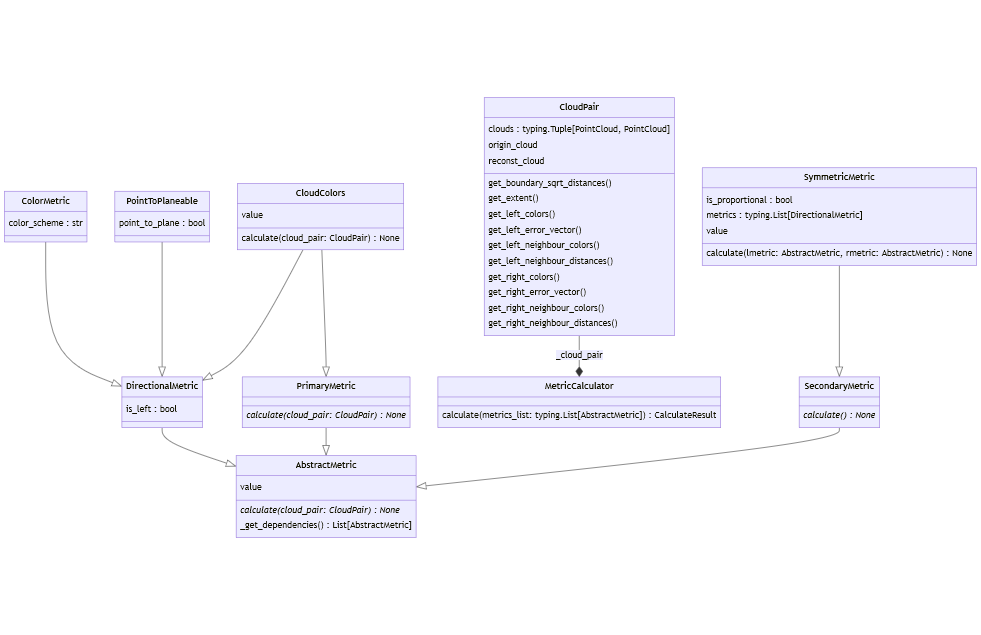
\includegraphics[width=0.7\linewidth]{assets/classes.png}
    \caption{Диаграмма классов разработанного приложения}
    \label{img:metric_classes}
\end{figure}

Диаграмма классов разработанного приложения приведена на рисунке
\ref{img:metric_classes}. Здесь непосредственно классом, который содержит в себе
оригинальное и реконструированное облака точек, а также другую информацию,
необходимую для сопоставления точек в данных облаках, является класс CloudPair.
Каждая метрика является наследником абстрактного класса AbstractMetric и
содержит ровно 2 метода: \texttt{calculate}, в котором реализован алгоритм
вычисления данной метрики, и служебный метод \texttt{\_get\_dependencies},
который возвращает зависимости данной метрики. Так, при подсчёте искажения
цвета, для PSNR (отношение пикового сигнала к шуму) зависимостью будет являться
MSE (среднеквадратичное отклонение). Класс MetricCalculator связывает между
собой отдельные метрики и объект CloudPair, благодаря чему снижается зависимость
данных классов между собой.

\paragraph{Алгоритм внедрения зависимостей}

\begin{lstlisting}[caption={
    Алгоритм подсчёта метрик.
}, label={lst:calculator_recursive_calculate}]
if metric._key() in self._calculated_metrics:
    return self._calculated_metrics[metric._key()]

if isinstance(metric, PrimaryMetric):
    metric = typing.cast(PrimaryMetric, metric)
    metric.calculate(self._cloud_pair)
    self._calculated_metrics[metric._key()] = metric
    return metric

calculated_deps = {}
for dep_key, dep_metric in metric._get_dependencies().items():
    calculated_dep_metric = self._metric_recursive_calculate(
        metric=dep_metric,
    )
    calculated_deps[dep_key] = calculated_dep_metric

metric.calculate(**calculated_deps)
self._calculated_metrics[metric._key()] = metric
\end{lstlisting}

На листинге \ref{lst:calculator_recursive_calculate} приведен алгоритм внедрения
зависимостей, позволяющий избежать повторного вычисления уже вычисленных метрик.
Данный алгоритм реализован в методе \texttt{recursive\_calculate} класса
MetricCalculator. В случае, если необходимая метрика уже вычислена, возвращается
вычисленное значение. Если метрика является первичной, то есть не имеет
зависимостей в виде других метрик, то в метод \texttt{calculate} метрики
передаётся объект CloudPair. Для вторичных метрик вызывается метод
\texttt{\_get\_dependencies}, при этом каждая из метрик-зависимостей передаётся
в метод \texttt{recursive\_calculate}, то есть рекурсивно применяется тот же
алгоритм.

\paragraph{Консольное приложение (help)}

\begin{figure}[H]
    \centering
    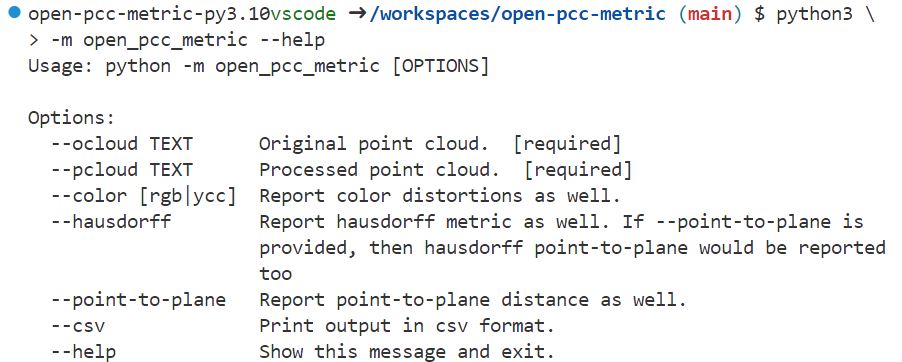
\includegraphics[width=0.7\linewidth]{assets/open_pcc_metric_help.png}
    \caption{Help-сообщение программы}
    \label{img:pcc_metric_help}
\end{figure}

Разработанное решение представляет собой консольное приложение. Help-сообщение
программы и входные параметры приведены на рисунке \ref{img:pcc_metric_help}. По
умолчанию программа выводит MSE и PSNR для координат точек, а также для цветов в
цветовой схеме RGB, клиент дополнительно может указать программе вычислить
метрику Хаусдорфа, значения метрик, проецированные вдоль нормалей (для MSE, PSNR
координат и метрики Хаусдорфа), а также указать цветовую схему, в которой должно
вычисляться искажение цветов. Дополнительно поддерживается вывод в формате CSV,
что может быть использовано при машинной обработке результатов.

\paragraph{Консольное приложение (вывод)}

\begin{figure}[H]
    \centering
    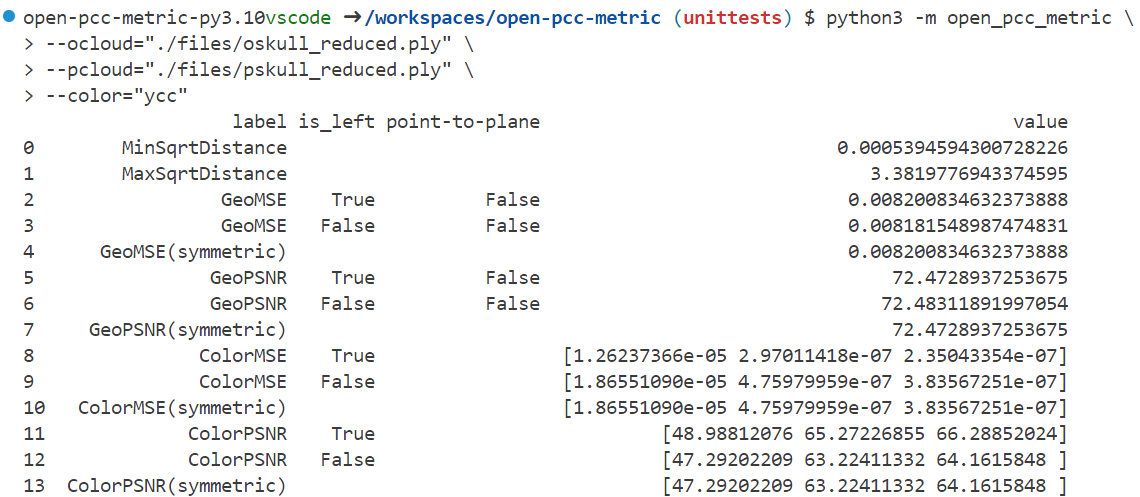
\includegraphics[width=0.7\linewidth]{assets/open_pcc_metric_output.png}
    \caption{Пример вывода программы}
    \label{img:pcc_metric_output}
\end{figure}

Пример работы программы приведен на рисунке \ref{img:pcc_metric_output}, здесь
отображены значения MSE и PSNR для координат и цветов, а также минимальное и
минимальное расстояние между парами точек в оригинальном и реконструированном
облаке.

\paragraph{Метрики разработанного ПО}

Тут про объем реализации (1к строк кода), тесты, CI/CD, много картинок, пару
красивых слов.

\paragraph{Тестовый пример (longdress)}

\begin{figure}[H]
    \centering
    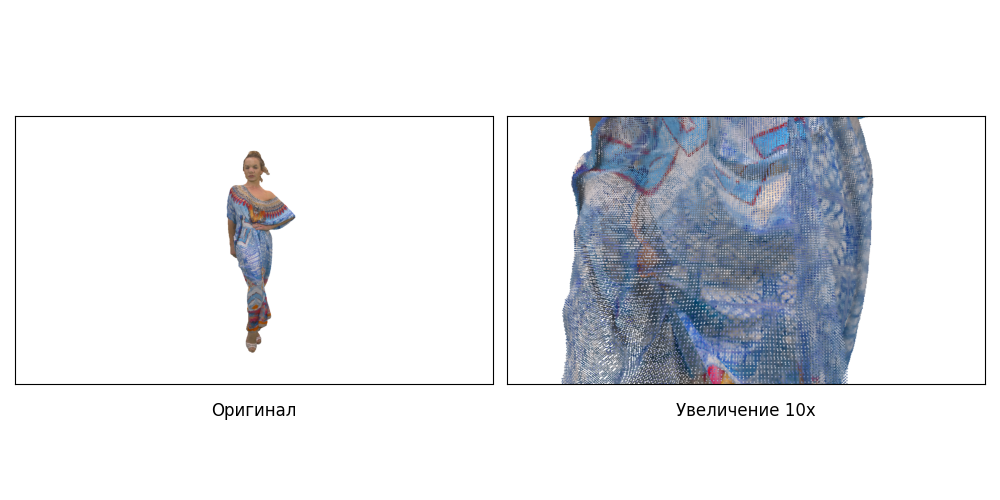
\includegraphics[width=0.7\linewidth]{assets/orig_plot.png}
    \caption{Оригинальное изображение и его увеличенная версия}
    \label{img:longdress_orig}
\end{figure}

Рассмотрим тестовый пример, представленный на рисунке \ref{img:longdress_orig},
подходящий для оценки искажения атрибутов облака точек. На слайде представлена
модель longdress, входящая в датасет 8iVFB. Облако точек данной модели было
сжато с помощью кодека TMC13 с помощью различных входных параметров.

\paragraph{Тестовый пример (longdress)}

\begin{figure}[H]
    \centering
    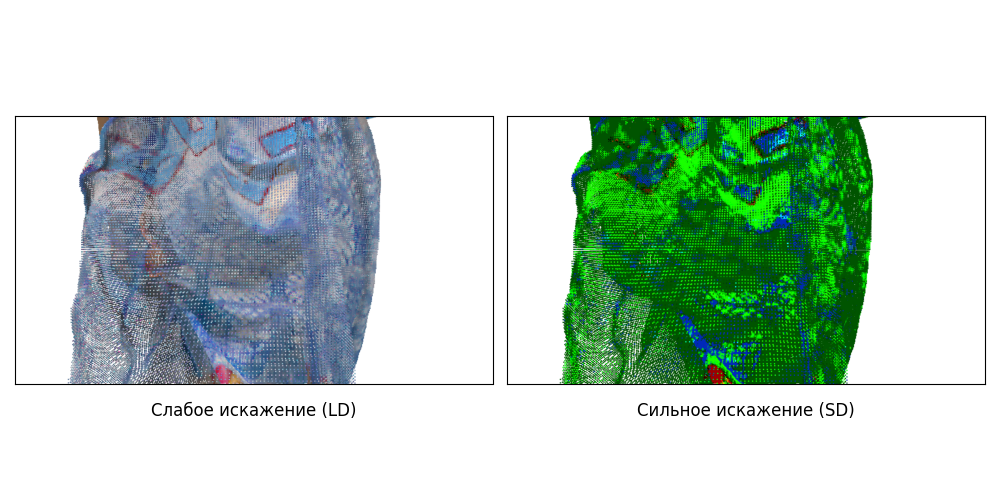
\includegraphics[width=0.7\linewidth]{assets/distorted_plot.png}
    \caption{Облака точек LD и SD}
    \label{img:longdress_dist}
\end{figure}

В результате были получены облака точек LD (Low Distortion) и SD (Severe
Distortion), представленные на рисунке \ref{img:longdress_dist}. (\textbf{для
SD, не читается:} qp=51, positionQuantizationScale=0.9375).

\paragraph{Введение про PCCArena}

Разработанное решение было внедрено в платформу PCCArena. PCCArena представляет
собой систему бенчмаркинга PCC-кодеков. Данная система использует
mpeg\_pcc\_dmetric для вычисления математически-обоснованные метрик (MSE, PSNR,
и т.д.), а также утилиту VMAF для оценки искажения более высокоуровневых
признаков облака путём предварительного рендеринга облака в изображение.

\paragraph{Архитектура PCCArena}

\begin{figure}[H]
    \centering
    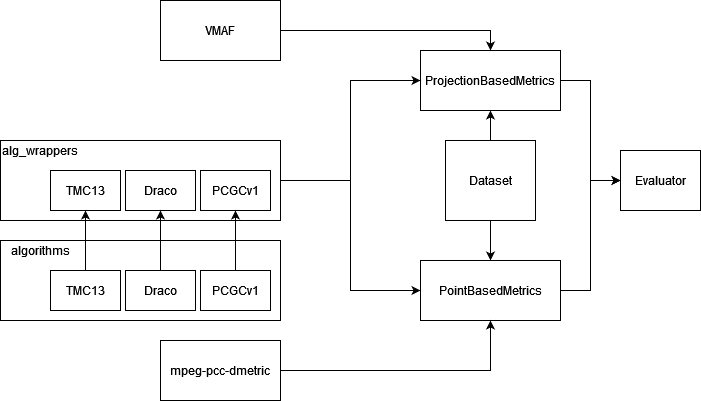
\includegraphics[width=0.7\linewidth]{assets/pcc_arena_architecture.png}
    \caption{Архитектура PCCArena}
    \label{img:pcc_arena_architecture}
\end{figure}

Архитектура PCCArena приведена на рисунке \ref{img:pcc_arena_architecture}. Для
внедрения разработанного решения в данную систему были внесены изменения в класс
PointBasedMetrics.

\paragraph{Описание проведенных экспериментов}

С помощью модифицированной системы PCCArena была произведена оценка кодеков
TMC13 и Draco, использовался датасет ShapeNet. Для каждой метрики строится
зависимость от битрейта - количества бит, затраченных на кодирование одной
точки.

\paragraph{Результаты для расстояния Чамфера}

\begin{figure}[H]
    \centering
    \begin{subfigure}{0.49\textwidth}
        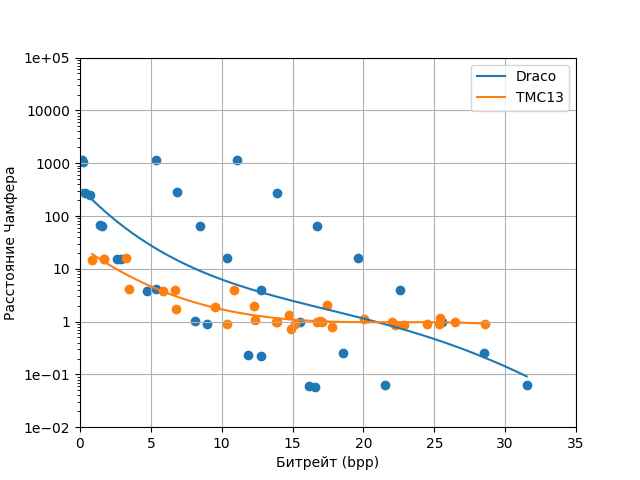
\includegraphics[width=\linewidth]{assets/approx_cd_p2pt.png}
        \caption{}
    \end{subfigure}
    \begin{subfigure}{0.49\textwidth}
        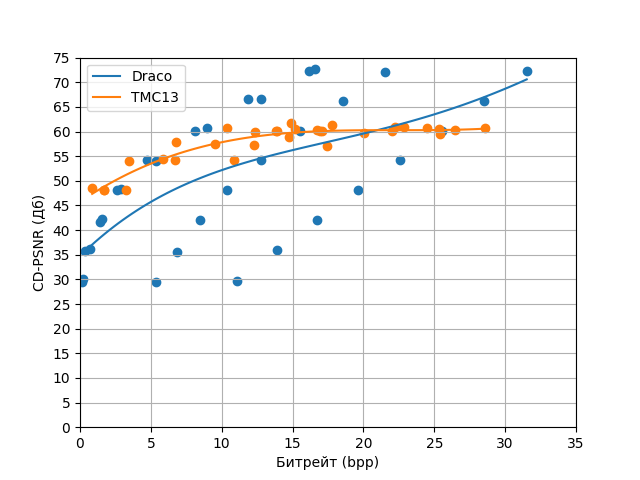
\includegraphics[width=\linewidth]{assets/approx_cdpsnr_p2pt.png}
        \caption{}
    \end{subfigure}
    \caption{ (a) Зависимость расстояния Чамфера от битрейта. (b) Зависимость
    CD-PSNR от битрейта. }
    \label{img:pcc_arena_cd_bpp}
\end{figure}


\paragraph{Результаты для метрики Хаусдорфа и нормалей}

\begin{figure}[H]
    \centering
    \begin{subfigure}{0.49\textwidth}
        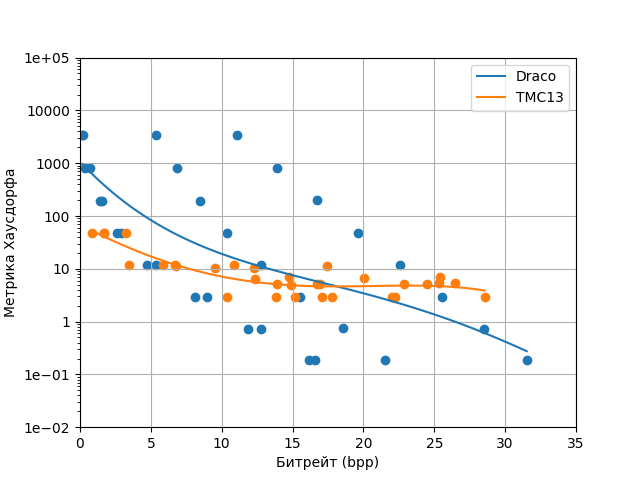
\includegraphics[width=\linewidth]{assets/approx_h_p2pt.png}
        \caption{}
    \end{subfigure}
    \begin{subfigure}{0.49\textwidth}
        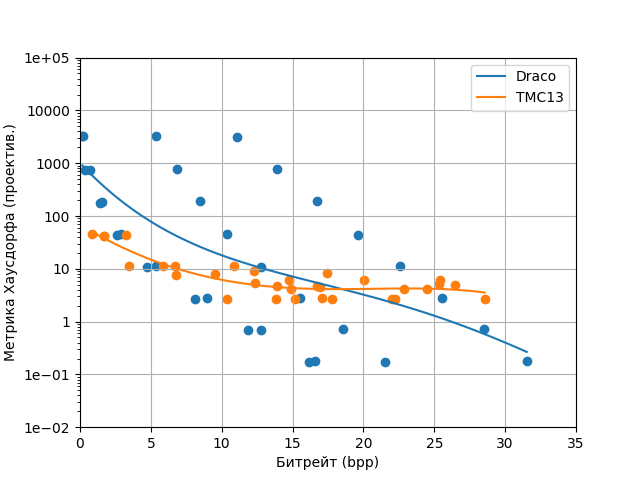
\includegraphics[width=\linewidth]{assets/approx_h_p2pl.png}
        \caption{}
    \end{subfigure}
    \caption{ (a) Зависимость метрики Хаусдорфа от битрейта. (b) Зависимость
    проецированной метрики Хаусдорфа от битрейта. }
    \label{img:pcc_arena_hd}
\end{figure}

\paragraph{Результаты для цветов}

\begin{figure}[H]
    \centering
    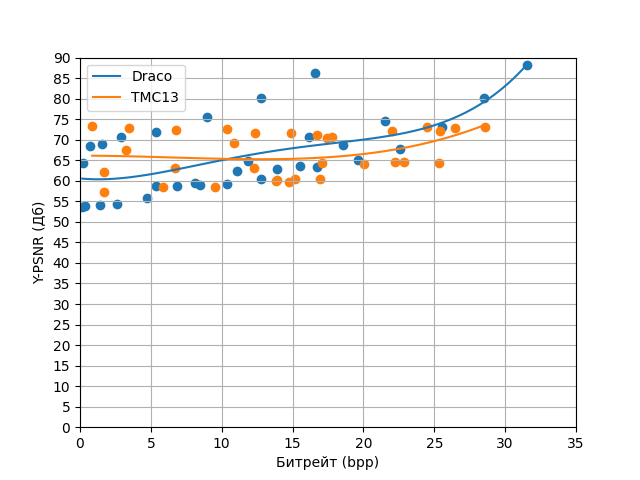
\includegraphics[width=0.49\linewidth]{assets/approx_y_psnr.png}
    \caption{ Зависимость Y'-PSNR от битрейта. }
    \label{img:pcc_arena_y_psnr}
\end{figure}

\paragraph{Выводы и дальнейшие шаги}

В данной работе был проведён анализ существующих систем оценки методов сжатия
облаков точек и их атрибутов. Разработана программа для оценки качества облака
точек при наличии оригинального облака точек. Произведён сравнительный анализ
кодеков Draco и TMC13. Полученные данные позволяют судить о качестве сжатия
облаков точек данными кодеками при различной степени сжатия. Разработанное
решение упростит оценку методов сжатия атрибутов облаков точек и может быть
полезным исследователям, ведущим разработки в данной области.

В рамках дальнейшей работы в программу могут быть добавлены метрики, учитывающие
более высокоуровневые признаки облаков точек и дающие более подробную оценку
качества их сжатия.

\subsection*{Extra. Метрики}

\noindent Метрика - мера, значение, полученное в результате измерения.

\noindent Метрика - ф-я, удовл. аксиомам тождества, симметричности и нер-ву
треугольника.


\end{document}